\chapter{Dynamic ARP Inspection}\label{dynamic-arp-inspection}

WHAT IS DYNAMIC ARP INSPECTION (DAI) ?

\section{ARP Review}\label{arp-review}

\begin{itemize}
\tightlist
\item
  ARP is used to learn the MAC ADDRESS of another DEVICE with a known IP
  ADDRESS

  \begin{itemize}
  \tightlist
  \item
    For example, a PC will use ARP to learn the MAC ADDRESS of its
    DEFAULT GATEWAY to communicate with external NETWORKS
  \end{itemize}
\item
  Typically, it is a TWO MESSAGE EXCHANGE : ARP REQUEST and ARP REPLY
\end{itemize}

\section{Gratuitous ARP}\label{gratuitous-arp}

\begin{itemize}
\tightlist
\item
  A GRATUITOUS ARP MESSAGE is an ARP REPLY that is sent without
  receiving an ARP REQUEST
\item
  It is SENT to the BROADCAST MAC ADDRESS
\item
  It allows other DEVICES to learn the MAC ADDRESS of the sending DEVICE
  without having to send ARP REQUESTS.
\item
  Some DEVICES automatically send GARP MESSAGES when an INTERFACE is
  enabled, IP ADDRESS is changed, MAC address is changed, etc.
\end{itemize}

\section{Dynamic ARP Inspection}\label{dynamic-arp-inspection-1}

\begin{itemize}
\tightlist
\item
  DAI is a SECURITY FEATURE of SWITCHES that is used to filter ARP
  MESSAGES received on \emph{UNTRUSTED PORTS}
\item
  DAI only filters ARP MESSAGES. Non-ARP MESSAGES are NOT affected
\item
  All PORTS are \emph{UNTRUSTED}, by DEFAULT

  \begin{itemize}
  \tightlist
  \item
    Typically, all PORTS connected to other NETWORK DEVICES (SWITCHES,
    ROUTERS) should be configured as TRUSTED, while INTERFACES connected
    to END HOSTS should remain UNTRUSTED
  \end{itemize}
\end{itemize}

\begin{figure}
\centering
\pandocbounded{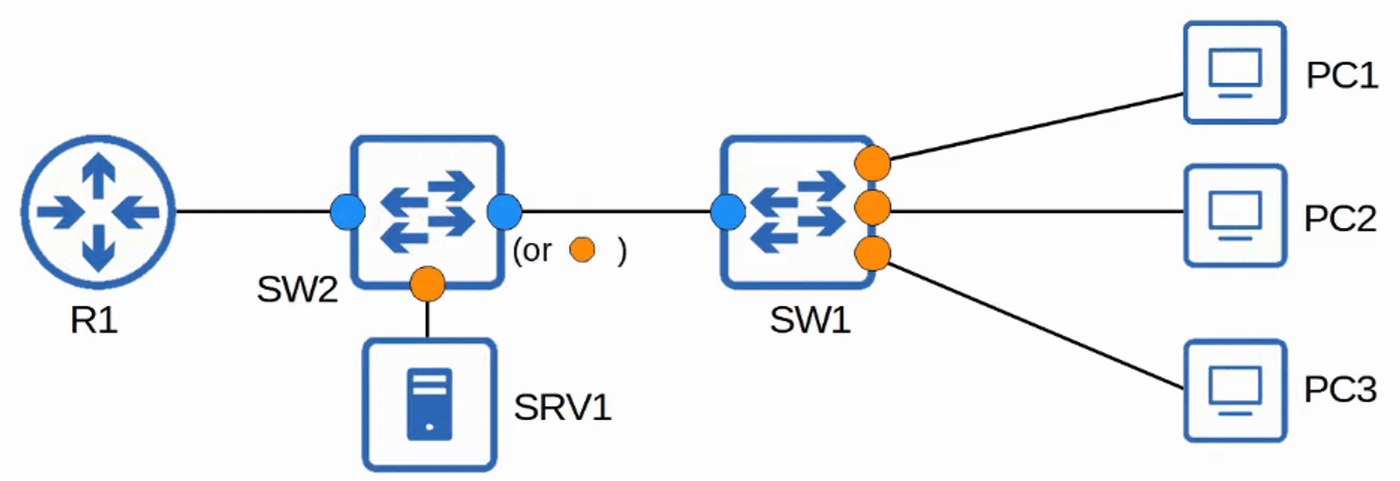
\includegraphics[keepaspectratio,alt={image}]{images/52-dynamic-arp-inspection/img-001.png}}
\end{figure}

\begin{figure}
\centering
\pandocbounded{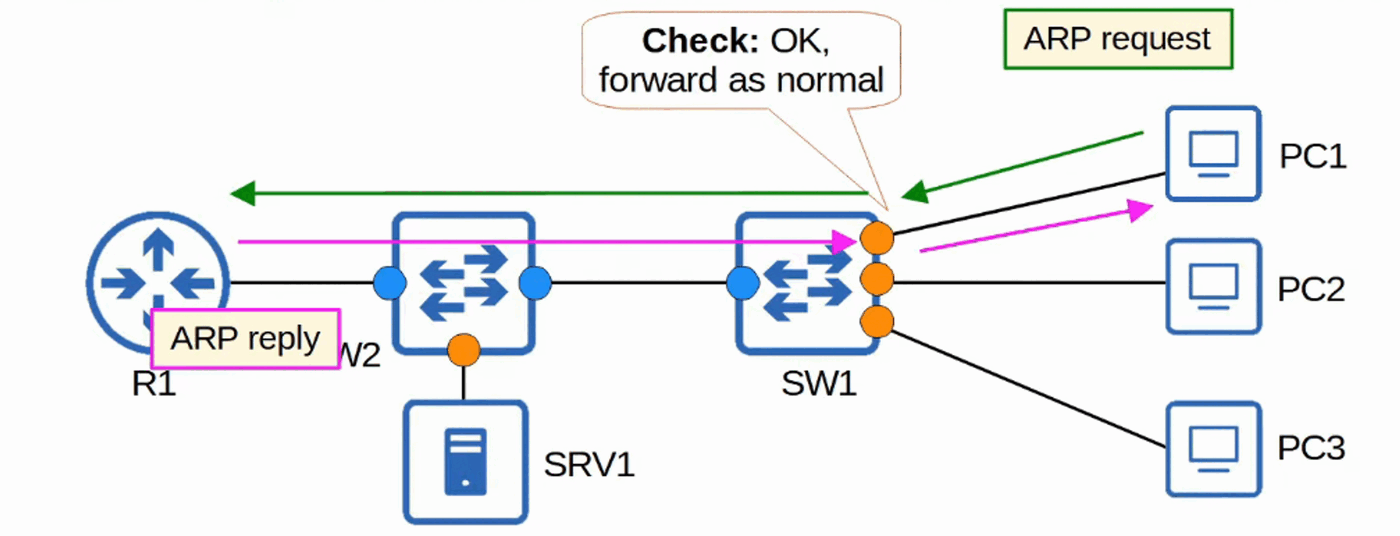
\includegraphics[keepaspectratio,alt={image}]{images/52-dynamic-arp-inspection/img-002.png}}
\end{figure}

\begin{figure}
\centering
\pandocbounded{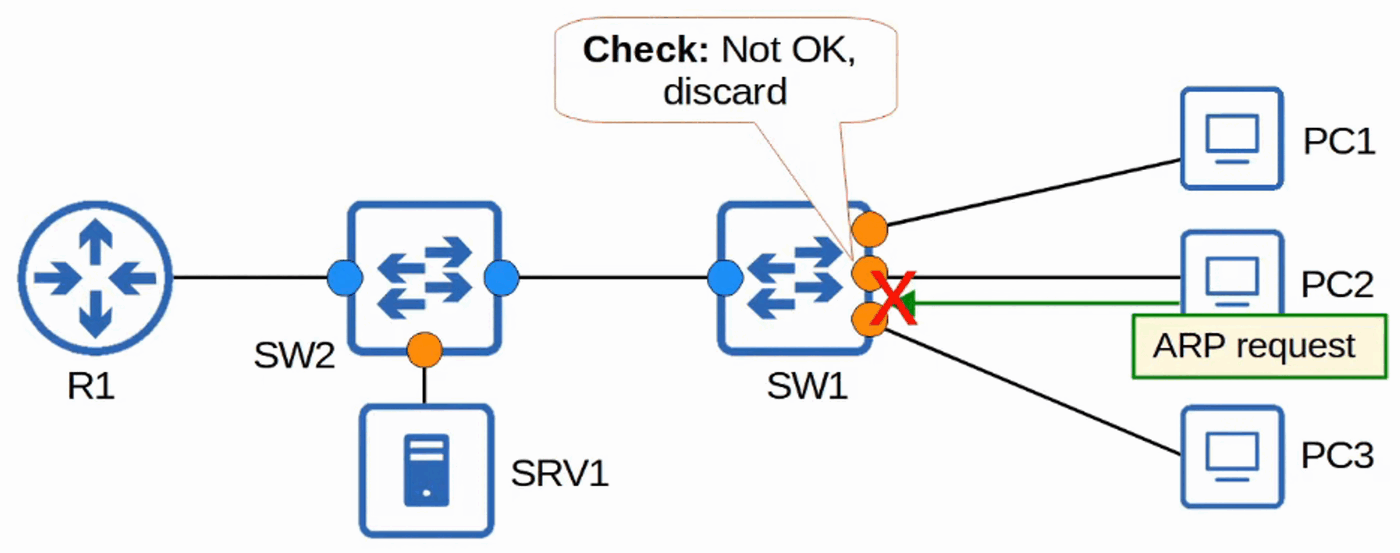
\includegraphics[keepaspectratio,alt={image}]{images/52-dynamic-arp-inspection/img-003.png}}
\end{figure}

\section{ARP Poisoning (Man in the
Middle)}\label{arp-poisoning-man-in-the-middle}

\begin{itemize}
\tightlist
\item
  Similar to DHCP POISONING, ARP POISONING involved an ATTACKER
  manipulating TARGET'S ARP TABLES so TRAFFIC is sent to the ATTACKER
\item
  To do this, the ATTACKER can send GRATUITOUS ARP MESSAGES using
  another DEVICE'S IP ADDRESS
\item
  Other DEVICES in the NETWORK will receive the GARP and update their
  ARP TABLES, causing them to send TRAFFIC to the ATTACKER instead of
  the legitimate DESTINATION
\end{itemize}

\begin{figure}
\centering
\pandocbounded{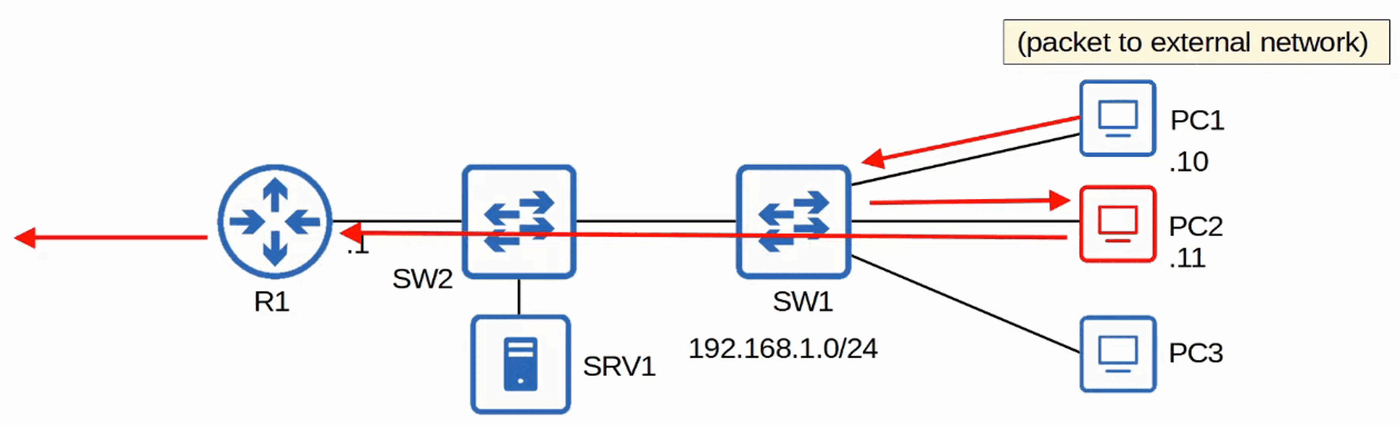
\includegraphics[keepaspectratio,alt={image}]{images/52-dynamic-arp-inspection/img-004.png}}
\end{figure}

\section{Dynamic ARP Inspection
Operations}\label{dynamic-arp-inspection-operations}

\begin{itemize}
\tightlist
\item
  DAI inspects the SENDER MAC and SENDER IP fields of ARP MESSAGES
  received on UNTRUSTED PORTS and checks that there is a matching entry
  in the DHCP SNOOPING BINDING TABLE

  \begin{itemize}
  \tightlist
  \item
    If there is a MATCH, the ARP MESSAGE is FORWARDED
  \item
    If there is NO MATCH, the ARP MESSAGE is DISCARDED
  \end{itemize}
\end{itemize}

\begin{figure}
\centering
\pandocbounded{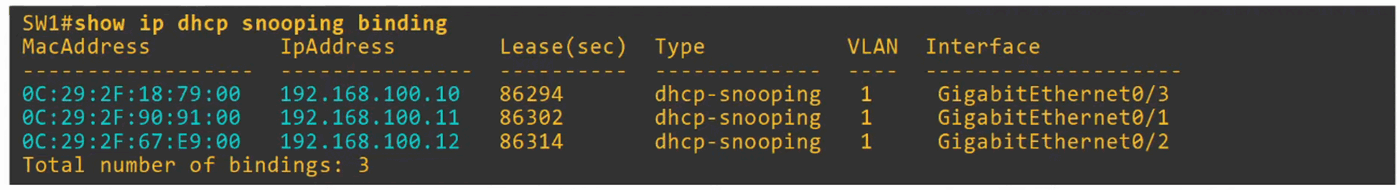
\includegraphics[keepaspectratio,alt={image}]{images/52-dynamic-arp-inspection/img-005.png}}
\end{figure}

\begin{itemize}
\item
  DAI doesn't inspect messages received on TRUSTED PORTS. They are
  FORWARDED as normal.
\item
  ARP ACLs can be manually configured to map IP ADDRESSES / MAC
  ADDRESSES for DAI to check

  \begin{itemize}
  \tightlist
  \item
    Useful for HOSTS that don't use DHCP
  \end{itemize}
\item
  DAI can be configured to perform more in-depth checks also - but these
  are optional
\item
  Like DHCP SNOOPING, DAI also supports RATE-LIMITING to prevent
  ATTACKERS from overwhelming the SWITCH with ARP MESSAGES

  \begin{itemize}
  \tightlist
  \item
    DHCP SNOOPING and DAI both require work from the SWITCH'S CPU
  \item
    Even if the ATTACKER'S messages are BLOCKED, they can OVERLOAD the
    SWITCH CPU with ARP MESSAGES
  \end{itemize}
\end{itemize}

\section{Dynamic ARP Inspection
Configuration}\label{dynamic-arp-inspection-configuration}

\begin{figure}
\centering
\pandocbounded{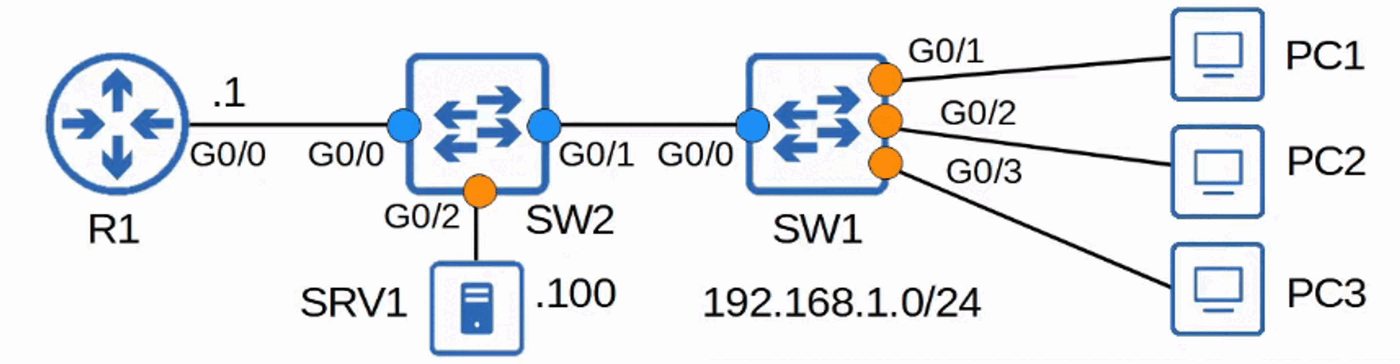
\includegraphics[keepaspectratio,alt={image}]{images/52-dynamic-arp-inspection/img-006.png}}
\end{figure}

\begin{figure}
\centering
\pandocbounded{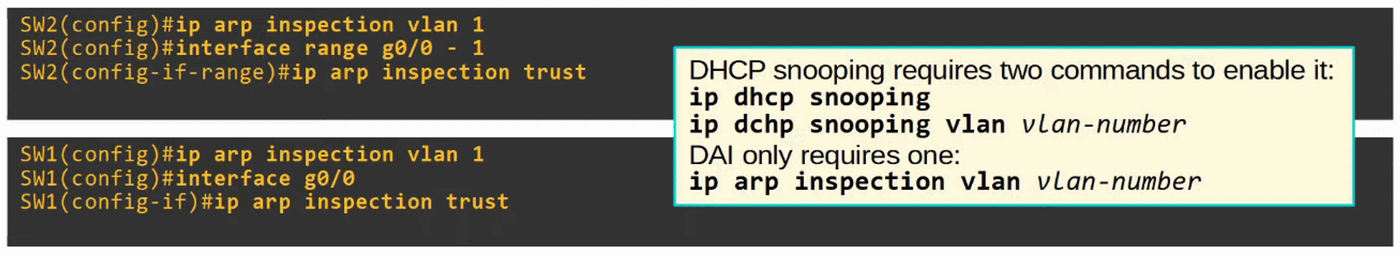
\includegraphics[keepaspectratio,alt={image}]{images/52-dynamic-arp-inspection/img-007.png}}
\end{figure}

Command : \passthrough{\lstinline!show ip arp inspection interfaces!}

\begin{figure}
\centering
\pandocbounded{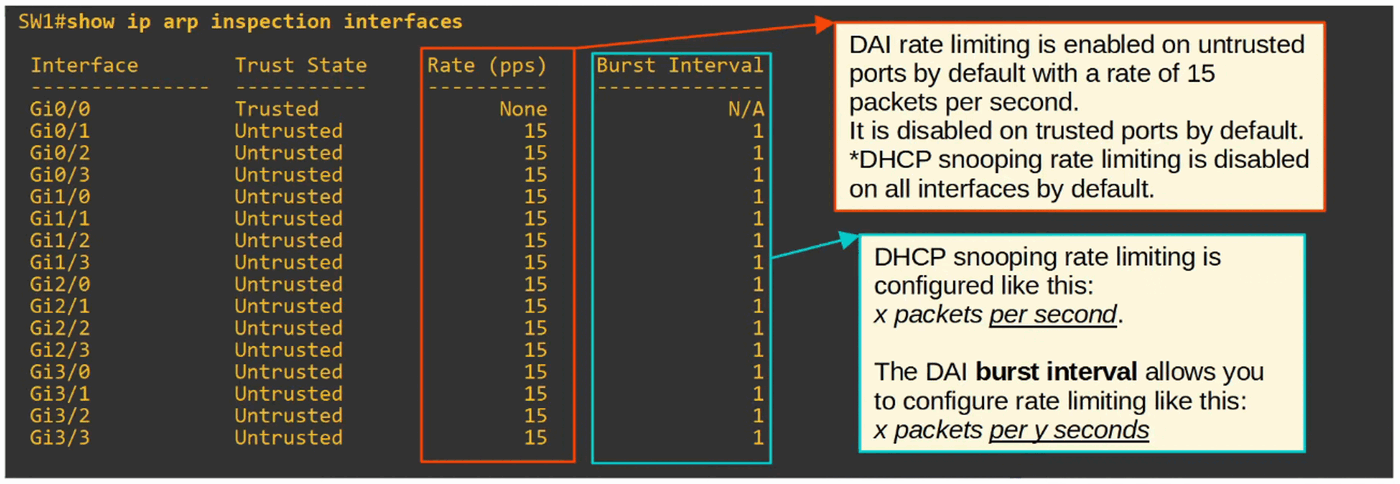
\includegraphics[keepaspectratio,alt={image}]{images/52-dynamic-arp-inspection/img-008.png}}
\end{figure}

\section{DAI Rate Limiting}\label{dai-rate-limiting}

\begin{figure}
\centering
\pandocbounded{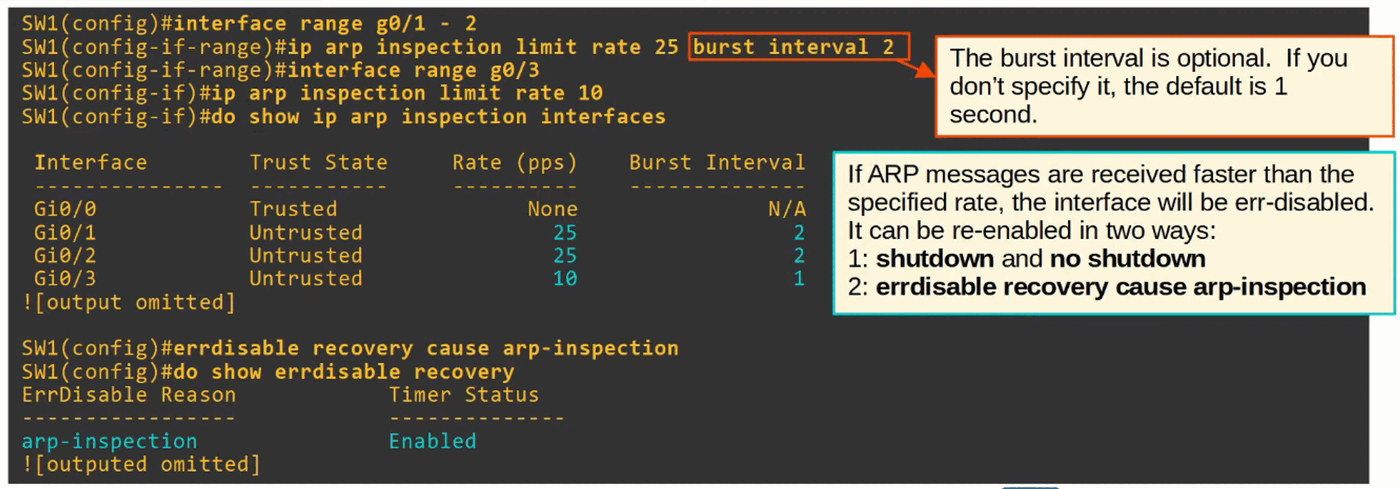
\includegraphics[keepaspectratio,alt={image}]{images/52-dynamic-arp-inspection/img-009.png}}
\end{figure}

\section{DAI Optional Checks}\label{dai-optional-checks}

\begin{figure}
\centering
\pandocbounded{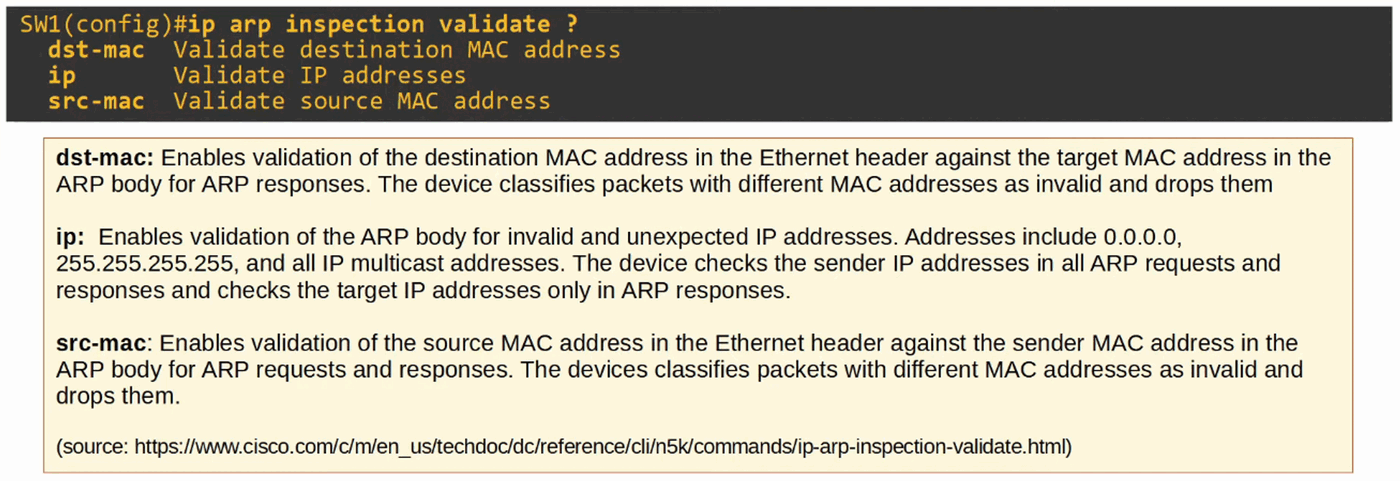
\includegraphics[keepaspectratio,alt={image}]{images/52-dynamic-arp-inspection/img-010.png}}
\end{figure}

\begin{figure}
\centering
\pandocbounded{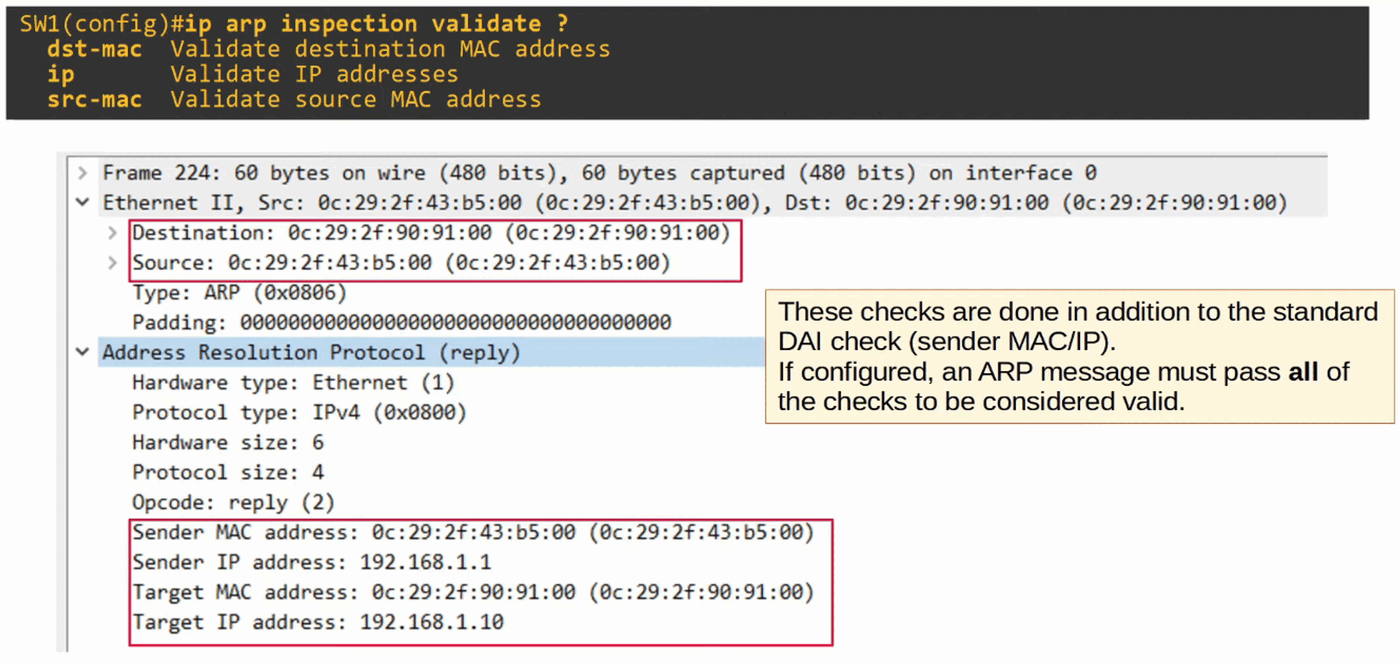
\includegraphics[keepaspectratio,alt={image}]{images/52-dynamic-arp-inspection/img-011.png}}
\end{figure}

\begin{figure}
\centering
\pandocbounded{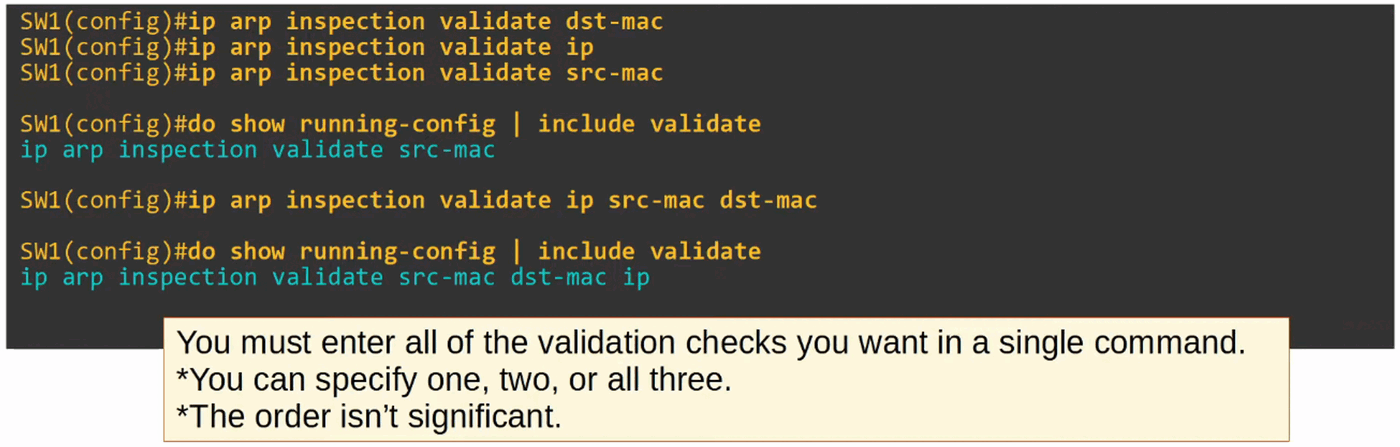
\includegraphics[keepaspectratio,alt={image}]{images/52-dynamic-arp-inspection/img-012.png}}
\end{figure}

ARP ACLs (Beyond Scope of CCNA)

\section{Create an ARP ACL for SRV1}\label{create-an-arp-acl-for-srv1}

\begin{figure}
\centering
\pandocbounded{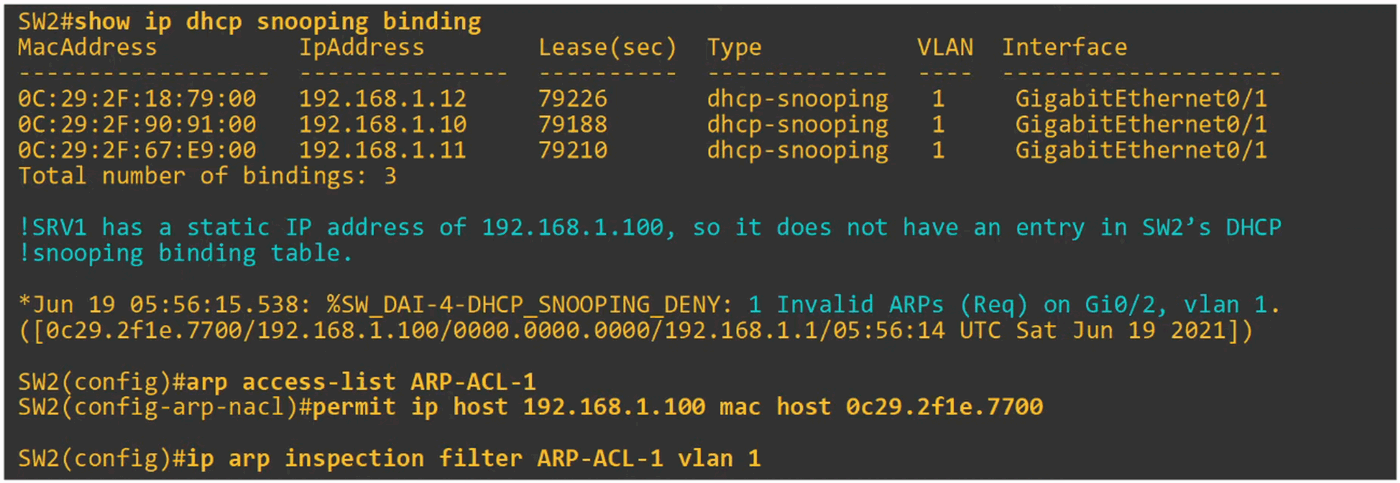
\includegraphics[keepaspectratio,alt={image}]{images/52-dynamic-arp-inspection/img-013.png}}
\end{figure}

AFTER APPLYING IT TO SWITCH 2, SRV1 is able to send ARP REQUEST to R1

\begin{figure}
\centering
\pandocbounded{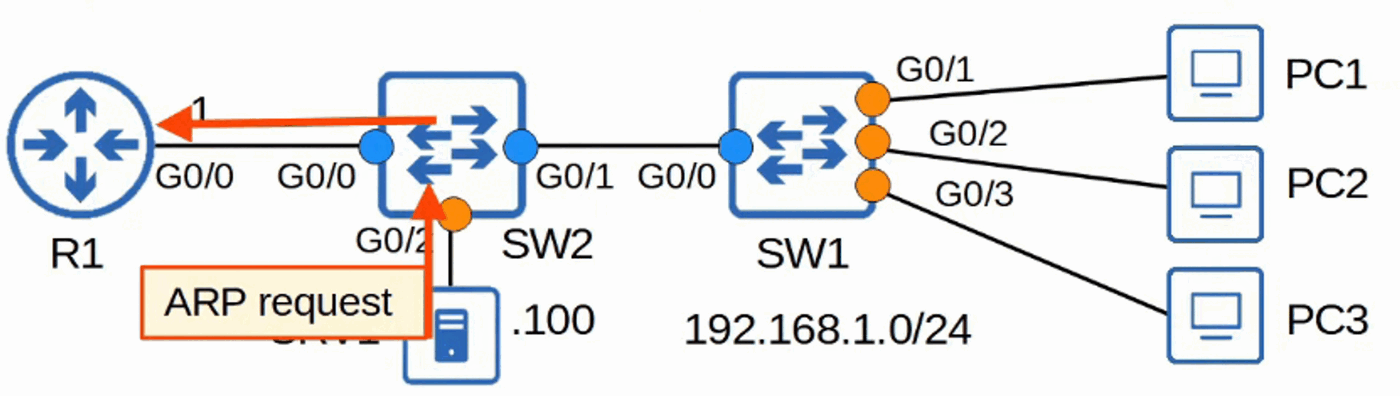
\includegraphics[keepaspectratio,alt={image}]{images/52-dynamic-arp-inspection/img-014.png}}
\end{figure}

Command: \passthrough{\lstinline!show ip arp inspection!}

Shows a summary of the DAI configuration and statistics

\begin{figure}
\centering
\pandocbounded{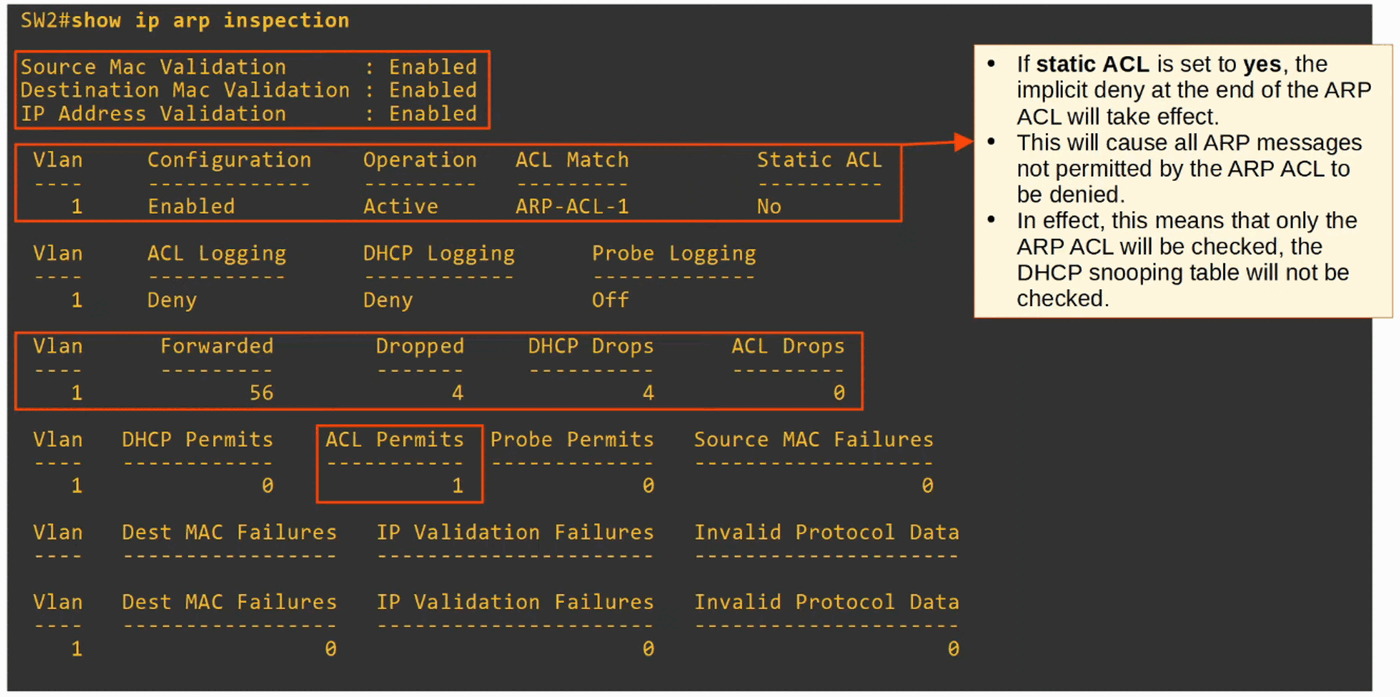
\includegraphics[keepaspectratio,alt={image}]{images/52-dynamic-arp-inspection/img-015.png}}
\end{figure}

\section{Command Review}\label{command-review}

\begin{figure}
\centering
\pandocbounded{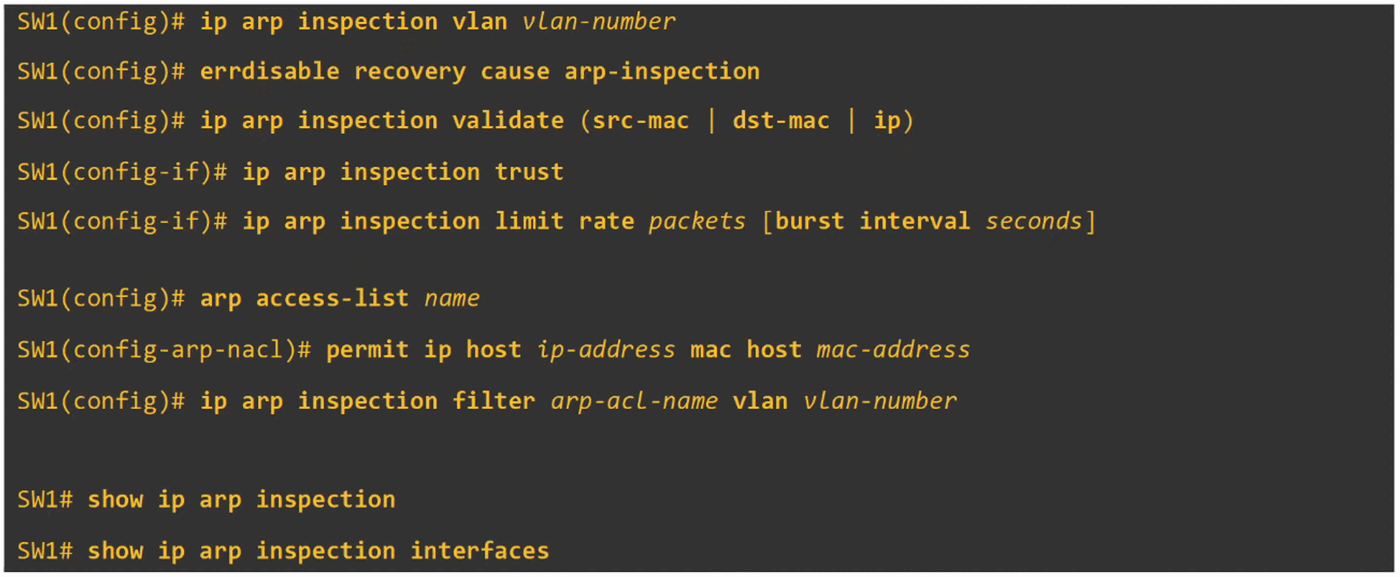
\includegraphics[keepaspectratio,alt={image}]{images/52-dynamic-arp-inspection/img-016.png}}
\end{figure}
